% Phases comparison report: nequip_no_zbl, nequip_zbl and rushik_zbl_pairwise against DFT-MD in the 8 DFT cells,
% and at 0 bar. Figures and every number from make_figures.py (figures/, metrics_compare.txt) and
% analysis/phases_npt.py (npt_compare.txt). Build: module load texlive/20220321; pdflatex phases_report.tex (twice).
\documentclass[11pt]{article}
\usepackage[margin=1in]{geometry}
\usepackage[T1]{fontenc}
\usepackage[utf8]{inputenc}
\usepackage{lmodern}
\usepackage{amsmath}
\usepackage{booktabs}
\usepackage{graphicx}
\usepackage{caption}
\usepackage{float}
\usepackage[hidelinks]{hyperref}
\captionsetup{font=small,labelfont=bf}
\graphicspath{{figures/}}
\newcommand{\GST}{Ge$_2$Sb$_2$Te$_5$}
\newcommand{\noz}{\texttt{nequip\_no\_zbl}}
\newcommand{\zbl}{\texttt{nequip\_zbl}}
\newcommand{\rzp}{\texttt{rushik\_zbl\_pairwise}}

\title{Three Allegro potentials for Ge--Sb--Te--C against DFT-MD:\\ structure, vibrations and density of the DFT phases}
\author{\texttt{cgst\_allegro\_sims}, \texttt{phases/report}}
\date{November 2026}

\begin{document}
\maketitle

\begin{abstract}
Three Allegro potentials, trained from scratch on the same PAW DFT data with the same settings and differing only in
their short-range term, were run in the eight cells of the 300\,K DFT molecular dynamics: amorphous \GST{} with 0,
1.4, 5.3 and 10\,at.\% C, and rocksalt and trigonal \GST{} with 0 and 1.4\% C. \noz{} has no short-range term,
\zbl{} a ZBL repulsion for every pair out to the 6\,\AA{} cutoff, and \rzp{} a per-pair ZBL at the edge of the
training data (1.15--1.76\,\AA). At the DFT volume (NVT) each potential reproduces the DFT radial distribution
(misfit $R$ 0.05--0.09), bond-angle distribution (overlap 0.92--0.98) and vibrational density of states (overlap
0.87--0.95), and the three potentials agree with each other more closely than any of them agrees with DFT: every
metric lies within about the scatter between seeds. They share the same deviations from DFT, too: Ge, Sb and Te
vibrate 1--10\% softer than in DFT in the amorphous cells, carbon 16--20\% stiffer in the 10\% C glass, and the
trigonal crystal has a sharp 2.9\,THz peak where DFT has a broad band. At 0\,bar (NPT) the rocksalt crystal is as
dense as the glass and the trigonal crystal about 1.5\% denser, for every potential. At 300\,K the short-range term
makes no measurable difference in these cells; where it can matter, in hot liquids and close contacts, is the subject
of the melt-quench comparison.
\end{abstract}

\section{Method}
The cells, the DFT references and the analysis are those of \texttt{phases/README.md}. Each potential ran each of
the 8 cells in NVT at the DFT volume, 300\,K Nos\'e--Hoover, 1\,fs, 5\,ps of equilibration and 20\,ps of production
dumped every step, three seeds per cell (the same seeds for every potential), as the DFT-MD was analysed. From the
trajectories, \texttt{analysis/phases\_compare.py} computes the total $g(r)$, the bond-angle distribution (ADF) with
the DFT files' bond cutoffs, and the vibrational density of states (VDOS) per atom with DoSPT, summed by species.
Metrics: the RDF misfit $R=\sqrt{\sum (g_A-g_D)^2/\sum g_D^2}$ over 1.5--6\,\AA{} (0 = identical); the ADF and VDOS
overlaps, the shared area of the two normalized curves (1 = identical); the mean frequency $\langle\nu\rangle$ of
the VDOS, total and per species. The amorphous cells were also analysed 20\,ps later (\texttt{\_eq25}), to see how
much the still-relaxing glass moves the metrics. Separately, the three C-free cells were run at 0\,bar (NPT, 500\,ps,
three seeds; isotropic for the glass, full cell relaxation for the crystals) for each potential's own density.

The checks pass for every potential: the DoSPT velocities equal the exact ones (overlap 1.0000), DoSPT's cell equals
the box in all 36 runs per potential, and the RDF/ADF code reproduces the DFT files from the DFT trajectory (ADF
overlap 0.9997). All metrics are mean $\pm$ sample standard deviation over the three seeds unless stated.

\begin{figure}[H]
\centering
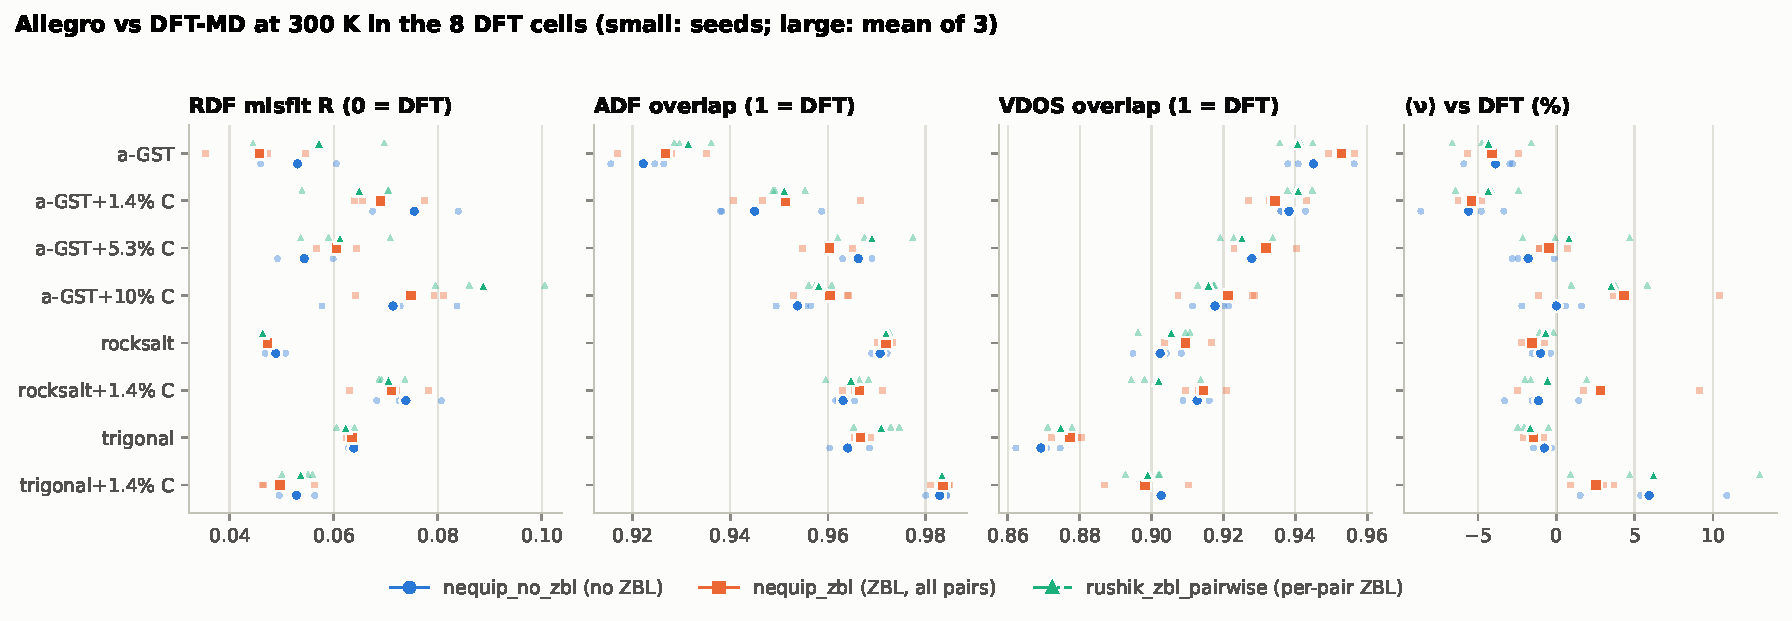
\includegraphics[width=\textwidth]{metrics_summary.pdf}
\caption{The four headline metrics per cell for the three potentials (small markers: seeds; large: mean). The
potentials overlap everywhere; the cells differ more from each other than the potentials do.}
\label{fig:summary}
\end{figure}

\begin{table}[H]
\centering
\caption{RDF misfit $R$, ADF overlap and total VDOS overlap against DFT-MD, mean of three seeds (seed standard
deviation in \texttt{metrics\_compare.txt}: 0.0003--0.013 for $R$, 0.001--0.014 for the overlaps).}
\label{tab:metrics}
\footnotesize\setlength{\tabcolsep}{4pt}
\begin{tabular}{l ccc ccc ccc}
\toprule
& \multicolumn{3}{c}{RDF misfit $R$} & \multicolumn{3}{c}{ADF overlap} & \multicolumn{3}{c}{VDOS overlap} \\
\cmidrule(lr){2-4}\cmidrule(lr){5-7}\cmidrule(lr){8-10}
cell & no ZBL & ZBL & pair & no ZBL & ZBL & pair & no ZBL & ZBL & pair \\
\midrule
amorphous GST       & 0.053 & 0.046 & 0.057 & 0.922 & 0.927 & 0.931 & 0.945 & 0.953 & 0.941 \\
amorphous + 1.4\% C & 0.075 & 0.069 & 0.065 & 0.945 & 0.951 & 0.951 & 0.938 & 0.934 & 0.941 \\
amorphous + 5.3\% C & 0.054 & 0.061 & 0.061 & 0.966 & 0.960 & 0.969 & 0.928 & 0.932 & 0.925 \\
amorphous + 10\% C  & 0.071 & 0.075 & 0.089 & 0.954 & 0.960 & 0.958 & 0.918 & 0.921 & 0.916 \\
rocksalt            & 0.049 & 0.047 & 0.046 & 0.971 & 0.972 & 0.972 & 0.902 & 0.910 & 0.906 \\
rocksalt + 1.4\% C  & 0.074 & 0.071 & 0.071 & 0.963 & 0.967 & 0.965 & 0.913 & 0.915 & 0.902 \\
trigonal            & 0.064 & 0.064 & 0.062 & 0.964 & 0.967 & 0.971 & 0.869 & 0.877 & 0.875 \\
trigonal + 1.4\% C  & 0.053 & 0.050 & 0.054 & 0.983 & 0.984 & 0.983 & 0.903 & 0.898 & 0.899 \\
\bottomrule
\end{tabular}
\\[2pt]{\footnotesize no ZBL = \noz, ZBL = \zbl, pair = \rzp.}
\end{table}

\section{Structure}
\begin{figure}[H]
\centering
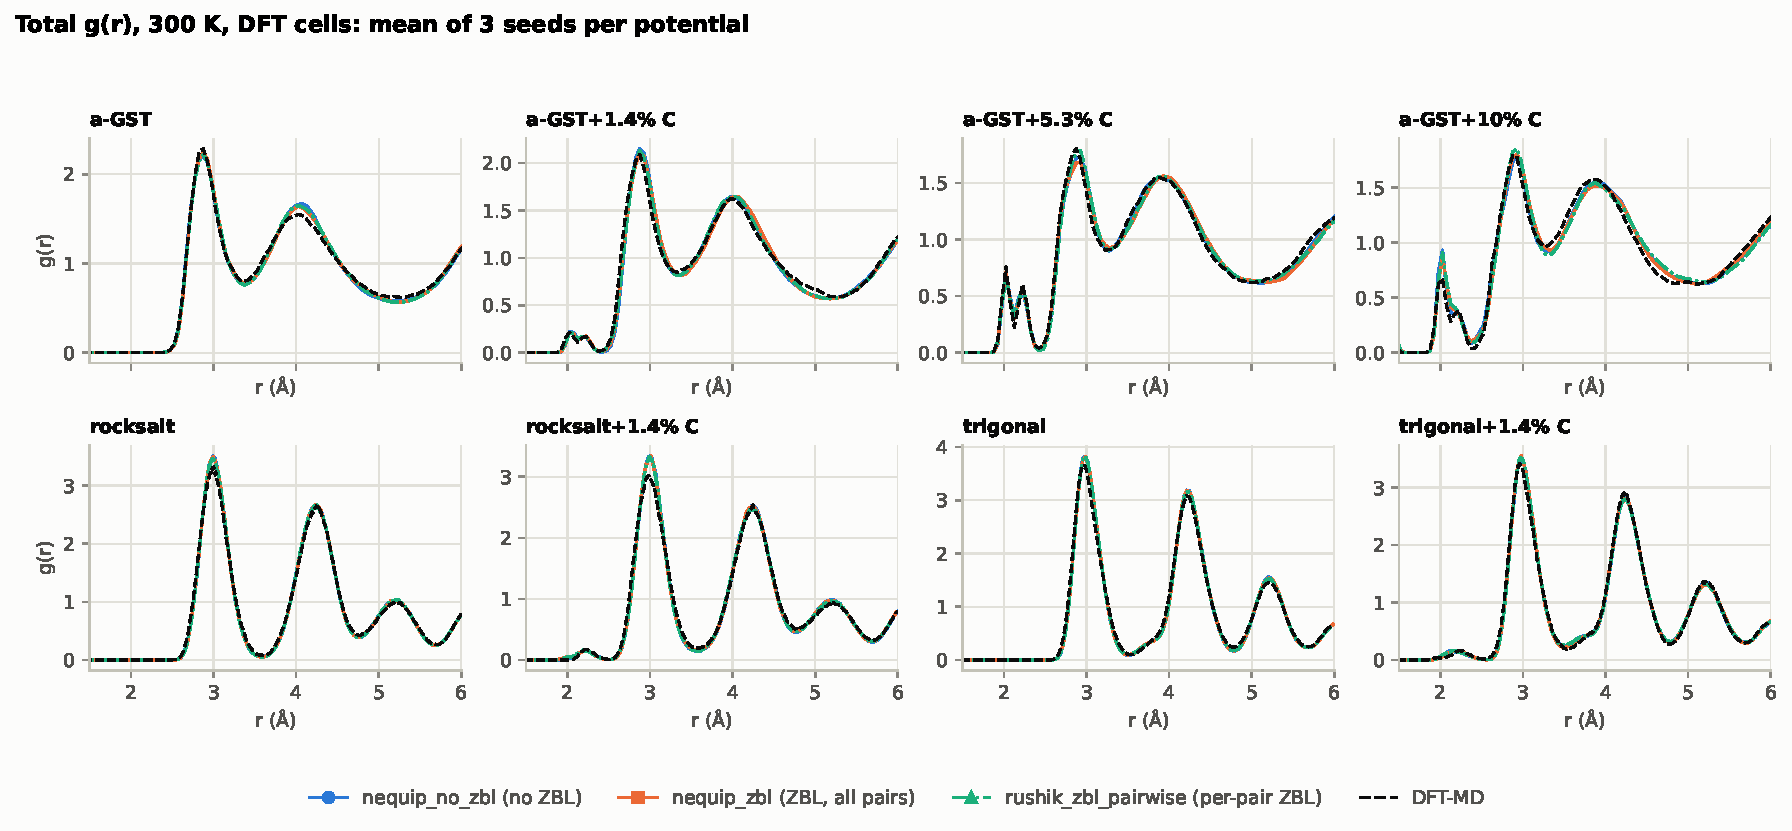
\includegraphics[width=\textwidth]{rdf_all.pdf}
\caption{Total $g(r)$ of the 8 cells, mean of three seeds per potential, and DFT-MD (dashed).}
\label{fig:rdf}
\end{figure}

The three $g(r)$ curves lie on top of each other in every cell (Fig.~\ref{fig:rdf}); their misfits to DFT differ by
less than the seed scatter (Table~\ref{tab:metrics}). In the crystals the first peak is 3--11\% taller than DFT's
(rocksalt 3.50 against 3.32, trigonal 3.82 against 3.66), for all three alike. The bond-angle distributions
(\texttt{figures/adf\_all}) agree as closely: ADF overlap 0.92--0.98, with the lowest values in amorphous GST, where
all three find 19\% fewer bond angles per atom than the DFT file (angles-per-frame ratio 0.80--0.82; the C-containing
glasses are within 3\% of DFT).

\begin{figure}[H]
\centering
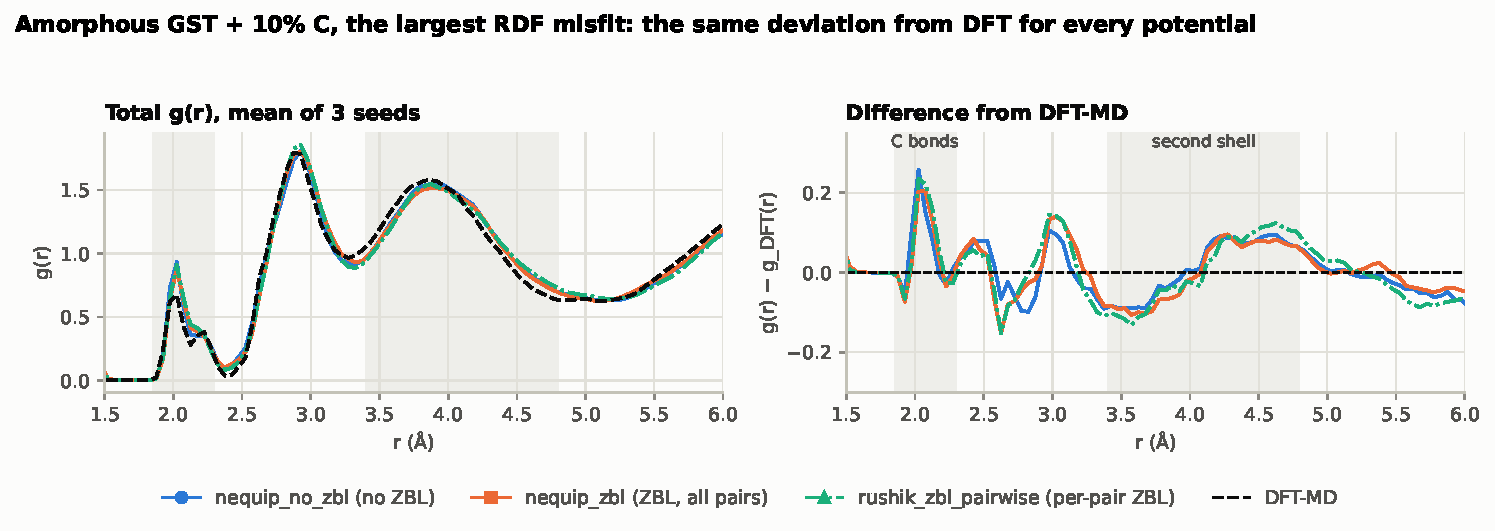
\includegraphics[width=\textwidth]{am_c10_detail.pdf}
\caption{Amorphous GST + 10\% C, the largest RDF misfit. Left: $g(r)$; right: difference from DFT-MD. Shaded: the
C--X bond region and the second shell.}
\label{fig:amc10}
\end{figure}

The largest misfit is in amorphous GST + 10\% C, where \rzp{} reads $R=0.089\pm0.006$ (standard error of the three
seeds) against $0.071\pm0.008$ (\noz) and $0.075\pm0.005$ (\zbl). The gap is under two standard errors, and the
deviation from DFT has the same shape for every potential (Fig.~\ref{fig:amc10}): the C-bond peak at 2.0\,\AA{} is
taller than DFT's ($g\approx0.9$ against 0.65), the valley before the second shell is lower, and the second shell
(3.4--4.8\,\AA) sits outward. The mean-of-seeds curves give $R$ = 0.067, 0.070 and 0.082.

\section{Vibrations}
\begin{figure}[H]
\centering
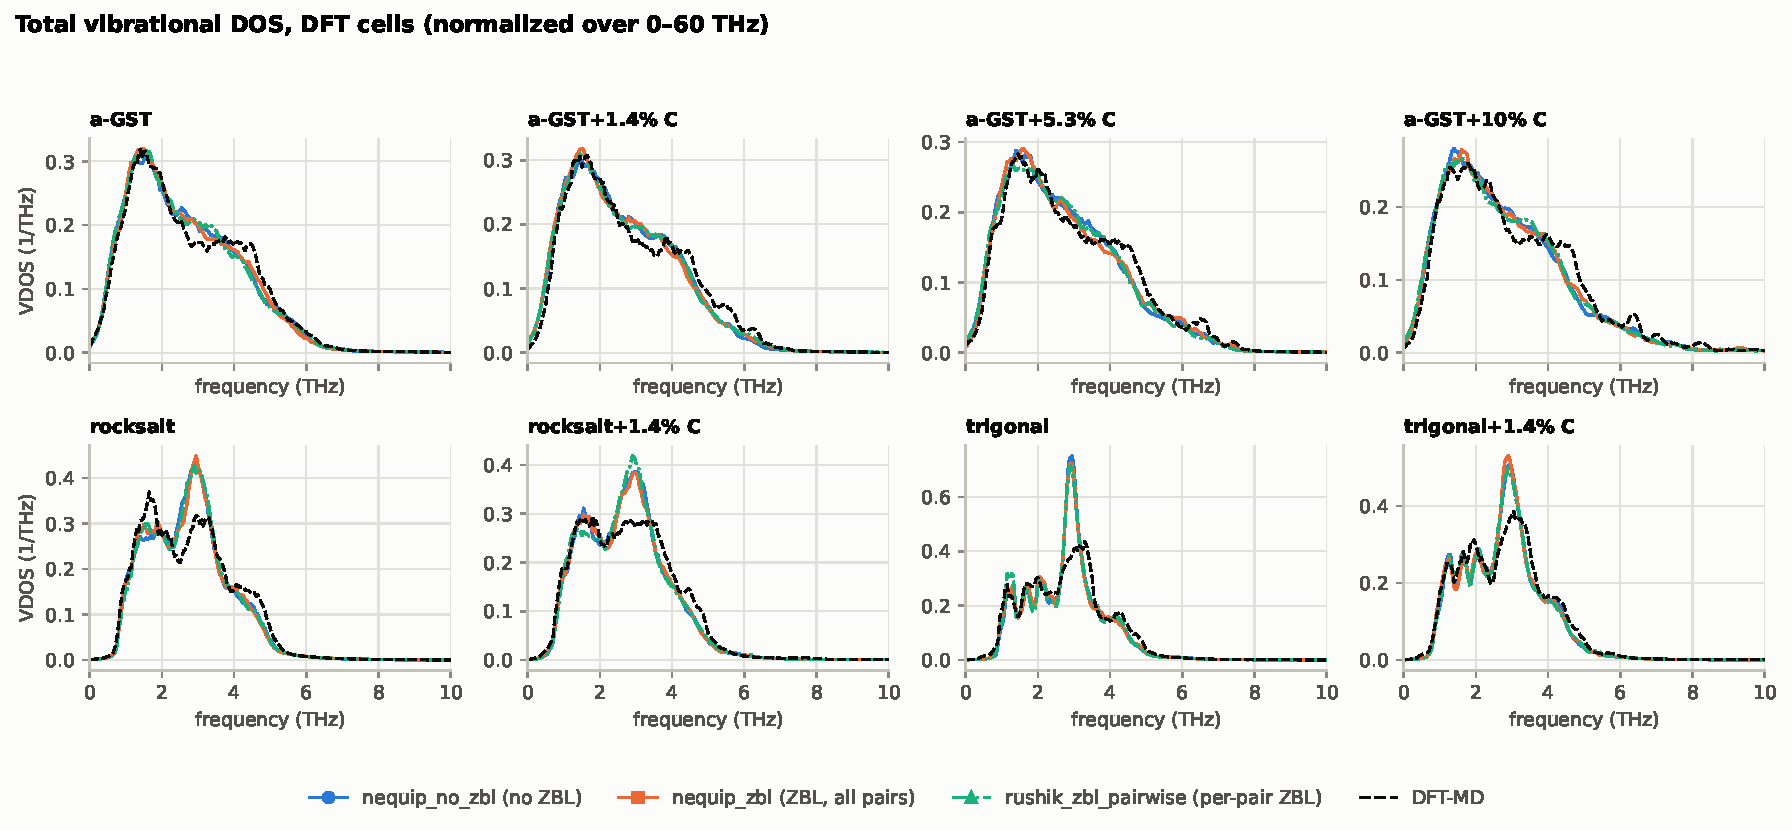
\includegraphics[width=\textwidth]{vdos_all.pdf}
\caption{Total VDOS of the 8 cells (each normalized over 0--60\,THz), mean of three seeds, and DFT-MD (dashed).}
\label{fig:vdos}
\end{figure}

\begin{figure}[H]
\centering
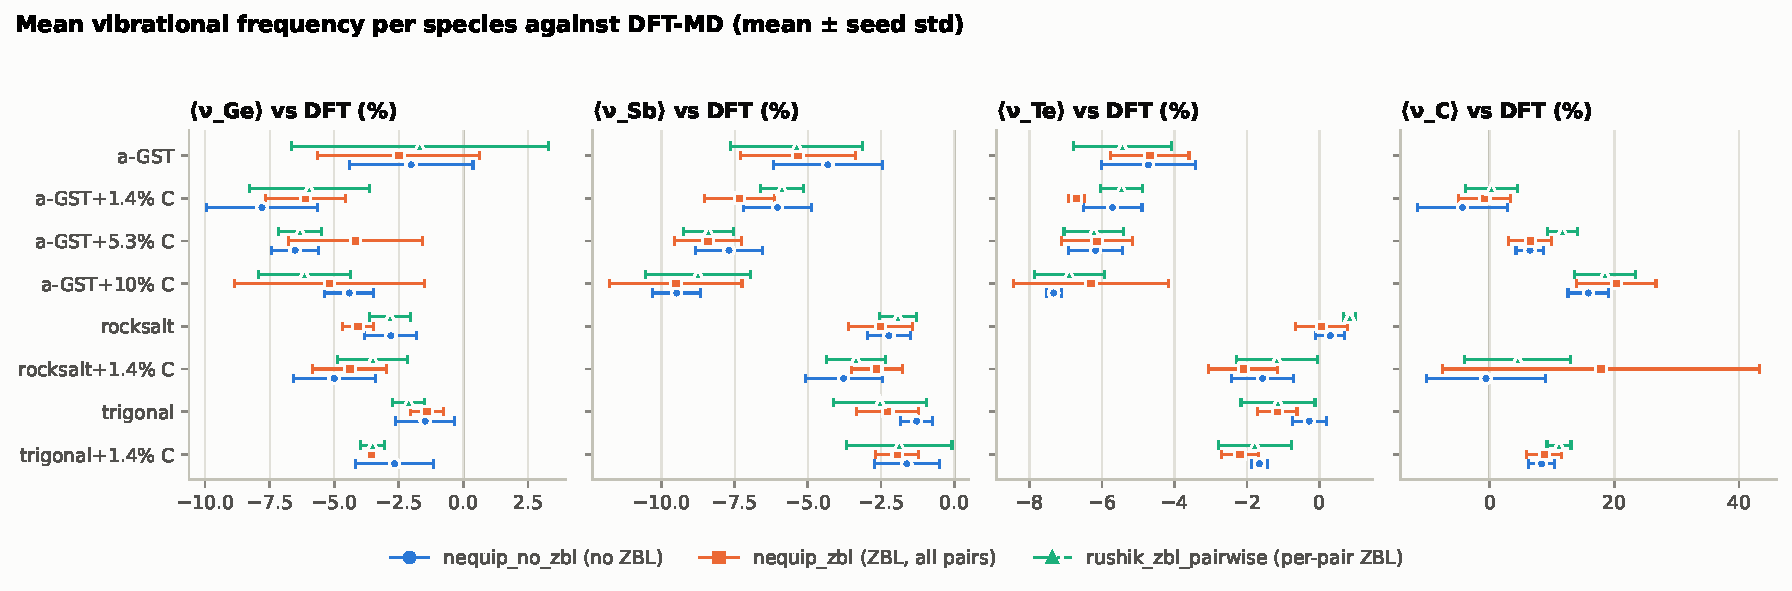
\includegraphics[width=\textwidth]{nu_species.pdf}
\caption{Mean frequency per species against DFT-MD (\%), mean $\pm$ seed standard deviation.}
\label{fig:nu}
\end{figure}

The total VDOS overlap is 0.87--0.95 for every potential (Table~\ref{tab:metrics}, Fig.~\ref{fig:vdos}). The
deviations are shared (Fig.~\ref{fig:nu}):
\begin{itemize}
\item \textbf{Ge, Sb and Te are soft in the amorphous cells,} by 1--10\% in mean frequency (most for Sb at 10\% C,
2.53--2.55 against 2.79\,THz), and within about 5\% in the crystals.
\item \textbf{The trigonal crystal} has a sharp Ge/Te peak near 2.9\,THz where DFT has a broad 2.6--3.4\,THz band: the
lowest VDOS overlap, 0.87--0.88, for all three potentials.
\item \textbf{Carbon} vibrates in the right bands, but its spectrum agrees least (Fig.~\ref{fig:cvdos}; C VDOS overlap
0.49--0.72). In the 10\% C glass the mean C frequency is 17.5--18.2\,THz against DFT's 15.1 (16--20\% high), for all
three. In rocksalt + 1.4\% C, two C atoms make the C metrics noisy (\zbl: 13.0 $\pm$ 2.8\,THz).
\end{itemize}

\begin{figure}[H]
\centering
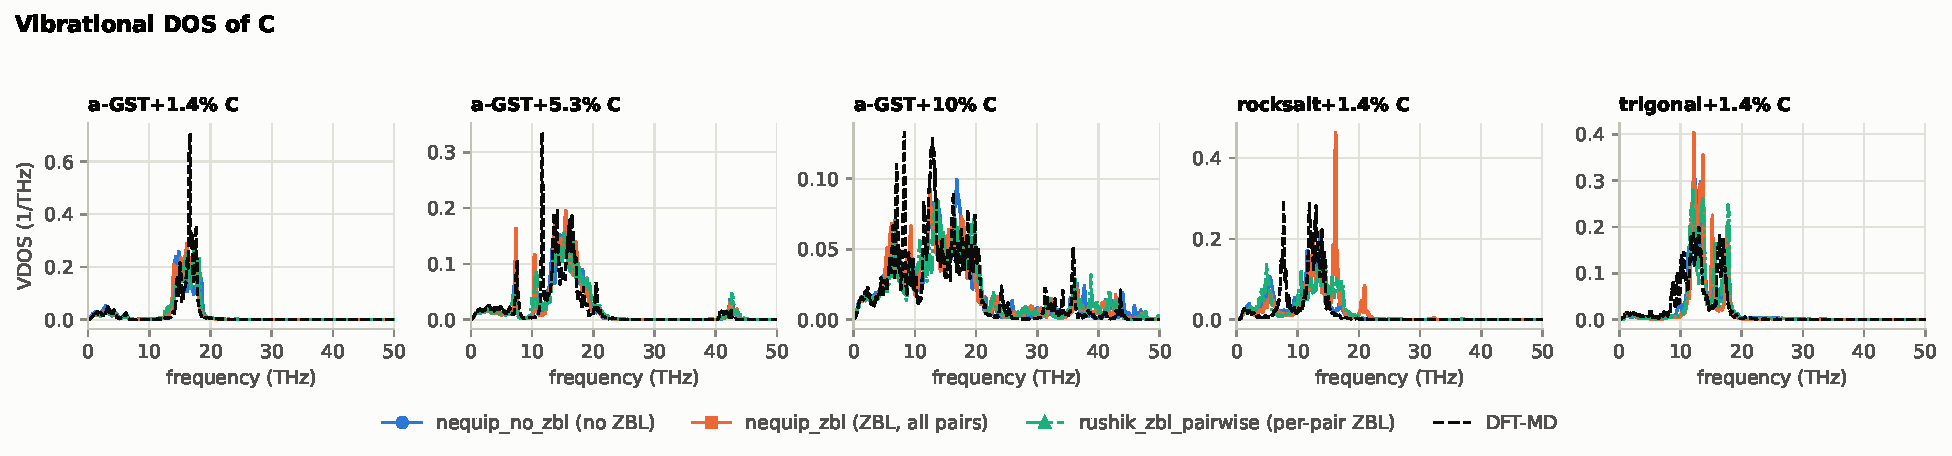
\includegraphics[width=\textwidth]{c_vdos.pdf}
\caption{VDOS of C in the five C-containing cells.}
\label{fig:cvdos}
\end{figure}

\section{Relaxation of the amorphous cells}
\begin{figure}[H]
\centering
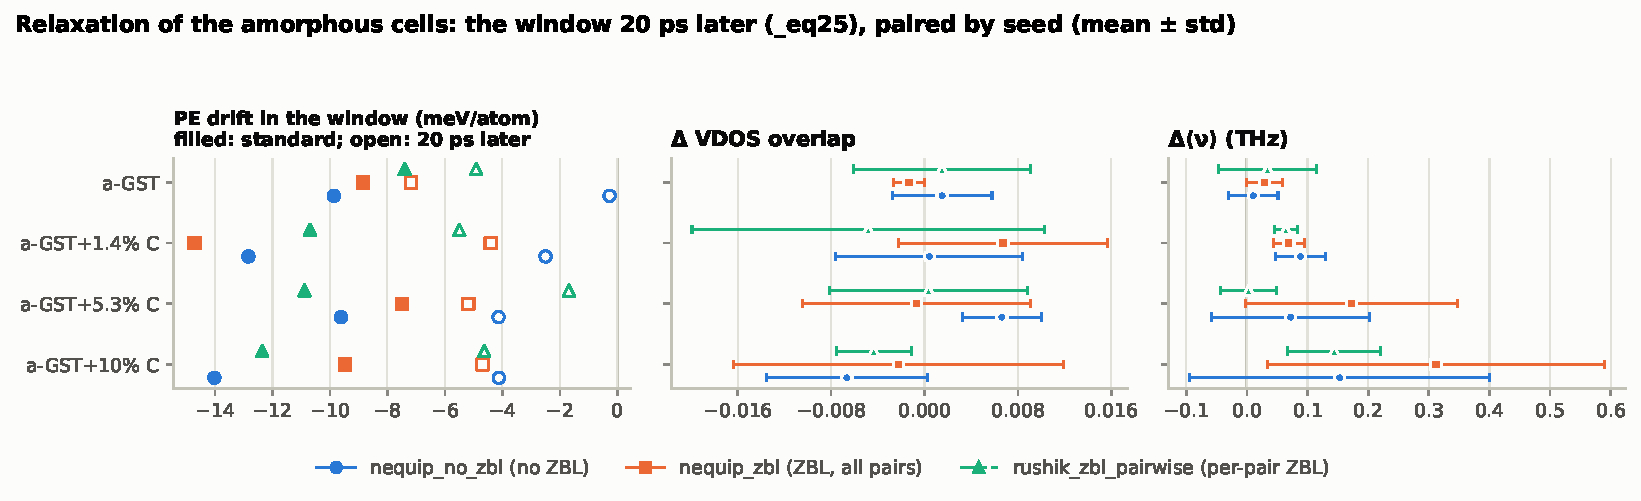
\includegraphics[width=\textwidth]{relaxation.pdf}
\caption{The amorphous cells analysed 20\,ps later (\texttt{\_eq25}), paired by seed. Left: potential-energy drift in
the 20\,ps window, standard (filled) and later (open). Middle and right: change of the total VDOS overlap and of
$\langle\nu\rangle$.}
\label{fig:relax}
\end{figure}

Every glass is still relaxing in the standard window (PE drift $-7$ to $-15$\,meV/atom over 20\,ps), and less 20\,ps
later ($-0.3$ to $-7$). The later window moves the VDOS overlap by at most 0.007 and $\langle\nu\rangle$ by up to
0.31\,THz (\zbl, 10\% C, with a paired seed scatter of 0.28), about the seed scatter or less (Fig.~\ref{fig:relax});
no conclusion above changes. The standard window, the one DFT used, remains the comparison.

\section{Density at 0 bar}
\begin{figure}[H]
\centering
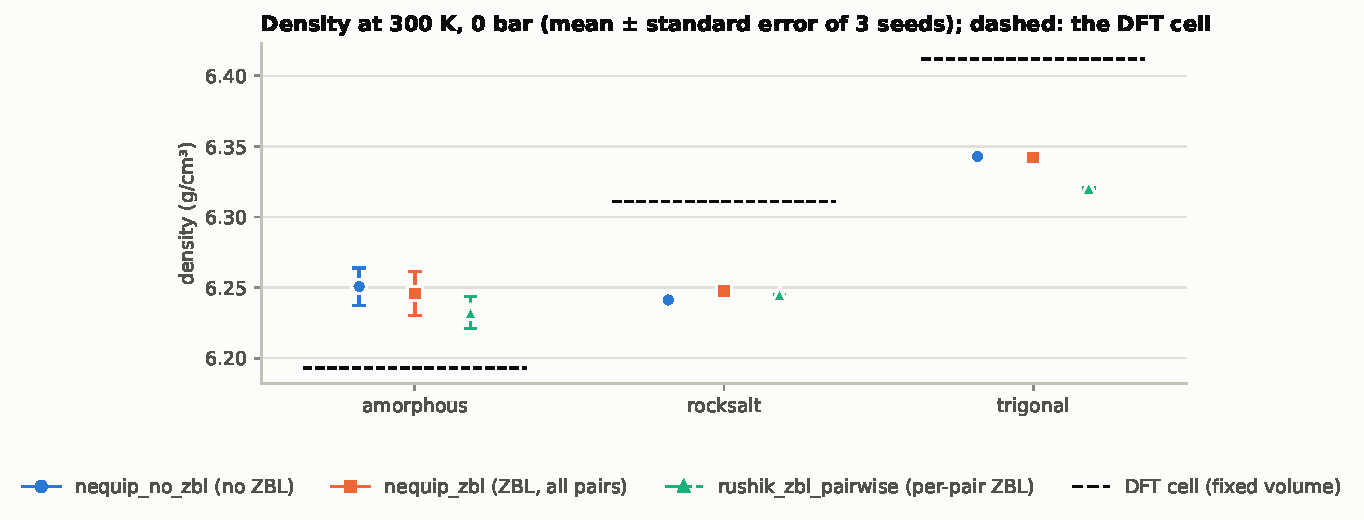
\includegraphics[width=0.8\textwidth]{npt_density.pdf}
\caption{Density at 300\,K and 0\,bar of the C-free cells (mean $\pm$ standard error of three seeds) and the density
of the DFT cell (dashed).}
\label{fig:npt}
\end{figure}

\begin{table}[H]
\centering
\caption{Density (g/cm$^3$) at 300\,K, 0\,bar, mean $\pm$ standard error of three seeds; crystal minus amorphous in
\% of the amorphous density. The DFT cells: amorphous 6.193, rocksalt 6.311, trigonal 6.412.}
\label{tab:npt}
\begin{tabular}{lccccc}
\toprule
potential & amorphous & rocksalt & trigonal & rocksalt $-$ am. & trigonal $-$ am. \\
\midrule
\noz & $6.251 \pm 0.013$ & 6.241 & 6.343 & $-0.15 \pm 0.21$\% & $+1.47 \pm 0.21$\% \\
\zbl & $6.246 \pm 0.016$ & 6.248 & 6.342 & $+0.03 \pm 0.25$\% & $+1.55 \pm 0.25$\% \\
\rzp & $6.232 \pm 0.011$ & 6.245 & 6.321 & $+0.20 \pm 0.18$\% & $+1.41 \pm 0.18$\% \\
\bottomrule
\end{tabular}
\end{table}

All three potentials give the same picture (Fig.~\ref{fig:npt}, Table~\ref{tab:npt}): the rocksalt crystal is as
dense as the glass, the trigonal crystal about 1.5\% denser. The DFT cells are not at the potentials' zero pressure:
the crystals expand by about 1\% and the glass contracts, so the DFT-cell gaps (rocksalt +1.9\%, trigonal +3.5\%)
mostly close. Experimentally amorphous GST is 6--7\% less dense than the crystal; the potentials follow their DFT
reference here, whose own melt-quenched glass is as dense as its crystal (\texttt{tests/dft\_glass}). The crystals
stay crystalline over 500\,ps; the glass seeds settle 0.02--0.03\,g/cm$^3$ apart and stay there, because a 144-atom
glass keeps its own structure at 300\,K.

\section{Conclusions}
\begin{itemize}
\item At 300\,K the three potentials are indistinguishable in the DFT cells: structure, angles and vibrations agree
with each other within the seed scatter and deviate from DFT in the same ways.
\item The short-range term (none, ZBL for all pairs, per-pair ZBL) makes no measurable difference at 300\,K: each
potential was fitted to the same data, and in these near-equilibrium cells the fit, not the short-range term,
decides the forces. Where it may matter is the hot liquid and close contacts (the melt-quench comparison, running).
\item The shared deviations, soft Ge/Sb/Te in the glasses, stiff C at 10\% C and the trigonal 2.9\,THz peak, come
from the shared training data and model form, not from the short-range term.
\end{itemize}

\section{Caveats}
\begin{itemize}
\item The DFT-MD of these cells is in the training data: this tests how the potentials reproduce their training
phases, not a prediction.
\item One DFT trajectory per cell; its own noise is unknown, and the $\pm$ are the potentials' seeds only.
\item $g(r)$ is compared to 6\,\AA; the DFT ADF files use Sb--Te cutoffs of 3.2 or 3.4\,\AA{} (matched per cell).
\item 144--160-atom cells; at 0\,bar the glass density depends on the seed by $\pm$0.03\,g/cm$^3$.
\end{itemize}

\end{document}
